\chapter{Đọc thêm 3: Massive Data Analytics for Macroeconomic Nowcasting}
\label{ch:M1L1-reading3}

\section{Phân tích Dữ liệu Lớn cho Dự báo Vĩ mô Hiện tại (Macroeconomic Nowcasting)}

\subsection{Ví dụ về Ứng dụng Vĩ mô Sử dụng Dữ liệu Lớn Thay thế}

Trong phần này, chúng tôi trình bày ba ví dụ sử dụng phương pháp luận mà chúng tôi đã phát triển nhằm dự báo (nowcast) tốc độ tăng trưởng của các tổng lượng vĩ mô sử dụng luồng thông tin đến từ các nguồn dữ liệu lớn thay thế. Các dự báo hiện tại cho tốc độ tăng trưởng của quý hiện tại được cập nhật mỗi khi có dữ liệu mới. Hóa ra là những dự báo vĩ mô này có lợi thế lớn là có sẵn rất lâu trước khi dữ liệu chính thức được công bố, đôi khi là vài tháng, trong khi vẫn cực kỳ đáng tin cậy. Ở một số quốc gia, nơi hệ thống thống kê chính thức còn yếu, các dự báo vĩ mô như vậy có thể bổ sung hiệu quả cho các chỉ số vĩ mô tiêu chuẩn để theo dõi hoạt động kinh tế.

\subsubsection{Một Biến đại diện Thời gian thực cho Xuất khẩu và Nhập khẩu}

\paragraph{Thương mại Quốc tế}
Có ba phương thức vận tải cho thương mại quốc tế: đường biển, đường hàng không và đường bộ. Mỗi phương thức vận tải sở hữu những ưu điểm và nhược điểm riêng dựa trên dịch vụ, lịch trình giao hàng, chi phí và mức độ tồn kho. Theo Transport and Logistics của Pháp, thị trường hàng hải chiếm khoảng 90\% thị trường xuất nhập khẩu nguyên liệu thô toàn cầu, với tổng số hơn 10 triệu tấn hàng hóa được giao dịch mỗi năm, theo UNCTAD [52]. Thật vậy, vận tải biển vẫn là cách rẻ nhất để chuyên chở nguyên liệu thô và sản phẩm. Ví dụ, nguyên liệu thô trong lĩnh vực năng lượng thống trị các lô hàng bằng đường biển với 45\% tổng số lô hàng. Theo sau là công nghiệp kim loại, chiếm 25\% tổng số, và sau đó là nông nghiệp, chiếm 13\%.

Các mặt hàng khác như dệt may, máy móc hoặc xe cộ chỉ chiếm 3\% phương tiện vận tải biển nhưng chiếm khoảng 50\% giá trị nguyên liệu thô được vận chuyển do giá trị cao của chúng. Tùy thuộc vào bản chất của chúng, nguyên liệu thô được vận chuyển trên các tàu chở hàng hoặc tàu chở dầu. Thật vậy, chúng ta thường đề cập đến bốn loại tàu chính: tàu đánh cá, tàu chở hàng (hàng khô), tàu chở dầu (hàng lỏng) và tàu ngoài khơi (các bộ phận khẩn cấp và bưu kiện nhỏ). Trong nghiên cứu của chúng tôi, chúng tôi sẽ chỉ tập trung vào các tàu chở hàng và tàu chở dầu vì chúng đại diện cho phần lớn nhất của khối lượng giao dịch bằng đường biển.

Trong phần tiếp theo, chúng tôi phát triển phương pháp luận để phân tích các chuyển động của tàu và tạo ra một biến đại diện (proxy) cho nhập khẩu và xuất khẩu đối với nhiều quốc gia và hàng hóa khác nhau.

\paragraph{Dữ liệu Vị trí (Localization Data)}
Chúng tôi lấy dữ liệu từ hệ thống nhận dạng tự động (AIS), phương pháp chính để tránh va chạm cho vận tải đường thủy. AIS tích hợp bộ thu phát VHF tiêu chuẩn với hệ thống định vị, chẳng hạn như bộ thu GPS, cũng như các cảm biến định vị điện tử khác, chẳng hạn như la bàn hồi chuyển. Các tàu được trang bị bộ thu phát AIS có thể được theo dõi bởi các trạm cơ sở AIS nằm dọc theo bờ biển hoặc, khi ra khỏi phạm vi của các mạng trên cạn, thông qua ngày càng nhiều vệ tinh được trang bị máy thu AIS đặc biệt có khả năng giải xung đột cho một lượng lớn tín hiệu. Về mặt này, chúng tôi có thể theo dõi hơn 70.000 tàu với bản cập nhật hàng ngày kể từ năm 2010.

\paragraph{Chỉ số Thương mại Quốc tế QuantCube: Trường hợp của Trung Quốc}
Chỉ số Thương mại Quốc tế QuantCube mà chúng tôi đã phát triển theo dõi sự phát triển của các con số thương mại đối ngoại chính thức trong thời gian thực bằng cách phân tích dữ liệu vận chuyển từ các cảng trên khắp thế giới và tính đến các đặc điểm của các tàu. Ví dụ, chúng tôi sẽ tập trung ở đây vào các trao đổi thương mại quốc tế của Trung Quốc, nhưng phương pháp luận của chỉ số thương mại quốc tế có thể được mở rộng sang nhiều quốc gia khác nhau và được điều chỉnh cho các mặt hàng cụ thể (dầu thô, than đá và quặng sắt).

Trước hết, chúng tôi thực hiện phân tích phương sai của xuất khẩu và nhập khẩu chính thức của Trung Quốc theo sản phẩm (xem Trade Map, dữ liệu hàng tháng 2005-2019). Hóa ra là (1) "máy móc và thiết bị điện" và "máy móc" chủ yếu giải thích phương sai của xuất khẩu của Trung Quốc và (2) "nhiên liệu khoáng, dầu và các sản phẩm", "máy móc và thiết bị điện" và "hàng hóa" chủ yếu giải thích phương sai của nhập khẩu của Trung Quốc.

Vì các sản phẩm đó được vận chuyển bằng tàu biển, chúng tôi đếm số lượng các loại tàu khác nhau cập bến tất cả các cảng của Trung Quốc. Thực tế, chúng tôi quan tâm đến ba loại tàu khác nhau: (1) tàu chở hàng rời (bulk cargo) vận chuyển hàng hóa, (2) tàu container vận chuyển máy móc thiết bị điện cũng như thiết bị và máy móc, và (3) tàu chở dầu (tanker) chở các sản phẩm dầu mỏ. Ví dụ, tổng số lượng tàu chở container cập cảng Trung Quốc mỗi ngày, từ tháng 7 năm 2012 đến tháng 7 năm 2019, được trình bày trong Hình 1. Các chuỗi thời gian hàng ngày tương tự cũng có sẵn cho tàu chở hàng rời và tàu chở dầu.

\begin{figure}[htbp]
    \centering
    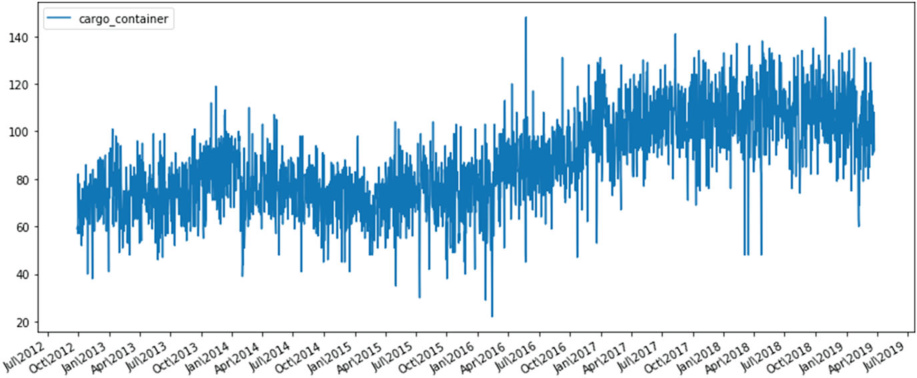
\includegraphics[width=0.8\textwidth]{gfx/m1l1_nowcast_cargo_container_index.jpg}
    \caption{Tổng số lượt cập bến của tàu container tại tất cả các cảng của Trung Quốc}
    \label{fig:nowcast_cargo_container_index}
\end{figure}

Để tránh sự biến động quá lớn trong dữ liệu hàng ngày, chúng tôi tính toán đường trung bình động (rolling average) trong 30 ngày của số lượng tàu thuộc ba loại đã chọn cập bến hàng ngày tại tất cả các cảng của Trung Quốc, như sau:
$$Ship_{(i,j)}^{q3}(t)=\frac{1}{30}\sum_{m=1}^{30}X_{i,j}(t-m)$$
với $X_{i,j}$ là số lượng tàu đến thuộc loại i [tàu container, tàu chở dầu, tàu chở hàng rời] tại một cảng j nhất định của Trung Quốc.

Cuối cùng, chúng tôi tính toán Chỉ số Thương mại Quốc tế QuantCube cho Trung Quốc sử dụng Phương trình (8) bằng cách cộng dồn ba loại hình vận chuyển và bằng cách tính toán những thay đổi so với cùng kỳ năm trước. Chỉ số này được thể hiện trong Hình 2. Chúng tôi nhận được mối tương quan là 80\% giữa Chỉ số Thương mại Quốc tế QuantCube theo thời gian thực và các con số thương mại chính thức của Trung Quốc (nhập khẩu + xuất khẩu). Đây là một chỉ số báo trước (leading index) 2 tháng do các con số chính thức về nhập khẩu và xuất khẩu hàng hóa được công bố với độ trễ 2 tháng sau khi kết thúc tháng tham chiếu. Chúng tôi nhận thấy chỉ báo của chúng ta chỉ ra rõ ràng tốc độ chậm lại của tổng thương mại Trung Quốc, chủ yếu bị tác động bởi số lượng gia tăng các lệnh trừng phạt thương mại của Mỹ kể từ giữa năm 2018.

\begin{figure}[htbp]
    \centering
    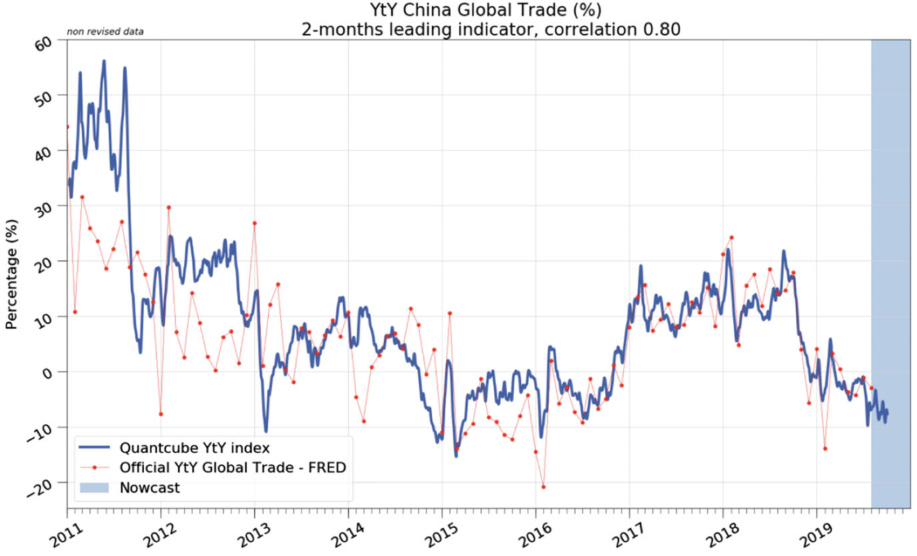
\includegraphics[width=0.8\textwidth]{gfx/m1l1_nowcast_china_trade_index.jpg}
    \caption{Chỉ số thương mại toàn cầu của Trung Quốc (tăng trưởng so với cùng kỳ năm trước tính bằng \%)}
    \label{fig:nowcast_china_trade_index}
\end{figure}

Đối với các quốc gia phụ thuộc nhiều vào các hoạt động trao đổi hàng hải, chỉ số này có thể đạt được mối tương quan với tổng các con số ngoại thương của quốc gia lên tới 95\%. Đối với các quốc gia chủ yếu dựa vào các giao dịch trên cạn, hóa ra chỉ số này vẫn là một biến đại diện tốt cho các trao đổi ở nước ngoài. Tuy nhiên, trong trường hợp sau, các biến đại diện của giao dịch qua đường hàng không và đường bộ có thể được tính toán để bổ sung thông tin, bằng cách sử dụng thông tin về các chuyến bay chở hàng hóa, phí cầu đường và lịch trình xe lửa.

\subsubsection{Một Biến đại diện Thời gian thực cho Tiêu dùng}

\paragraph{Tiêu dùng Cá nhân}
Khi theo dõi hoạt động kinh tế, tiêu dùng cá nhân (private consumption) là một tổng lượng vĩ mô quan trọng mà chúng ta cần đánh giá theo thời gian thực. Ví dụ, ở Mỹ, tiêu dùng cá nhân chiếm khoảng 70\% tăng trưởng GDP. Vì các con số chính thức về tiêu dùng cá nhân được công bố hàng tháng (ví dụ: ở Mỹ) hoặc hàng quý (ví dụ: ở Trung Quốc) và với độ trễ công bố từ 1 đến 3 tháng, các nguồn dữ liệu thay thế, chẳng hạn như Google Trends, có thể truyền tải thông tin hữu ích khi thiếu thông tin chính thức.

Vì chi tiêu cá nhân nằm trong các nhóm hàng hóa lâu bền, hàng hóa không lâu bền và dịch vụ, trước tiên chúng tôi tiến hành phân tích phương sai của tiêu dùng đối với các quốc gia được nghiên cứu, để làm nổi bật các thành phần chính của tiêu dùng mà chúng ta phải theo dõi. Ví dụ, đối với tiêu dùng của Trung Quốc, chúng tôi đã xác định các danh mục sau: Đồ xa xỉ (túi xách, đồng hồ, rượu vang, đồ trang sức), Bán lẻ (thực phẩm, đồ uống, quần áo, thuốc lá, điện thoại thông minh, máy tính, đồ điện tử), Phương tiện, Dịch vụ (khách sạn, khoản vay tín dụng, phương tiện đi lại) và Giải trí (du lịch, thể thao, điện ảnh, chơi game). Trong phần này, chúng tôi tập trung vào một chỉ số phụ (sub-indicator) của biến đại diện cho tiêu dùng Trung Quốc của QuantCube, đó là Du lịch (thuộc danh mục Giải trí). Phương pháp tương tự cũng được phát triển để theo dõi các thành phần chính khác của tiêu dùng hộ gia đình.

\paragraph{Nguồn Dữ liệu Thay thế}
Thành phần phụ du lịch của tiêu dùng Trung Quốc được cho là để theo dõi chi tiêu của người dân Trung Quốc cho các chuyến đi du lịch, trong và ngoài nước. Để tạo ra thành phần phụ này của chỉ số tiêu dùng, chúng tôi đã sử dụng các truy vấn tìm kiếm liên quan đến du lịch được trích xuất thông qua các ứng dụng Google Trends và Baidu. Trên thực tế, các truy vấn tìm kiếm trên Internet có sẵn thông qua Google Trends và Baidu cho phép chúng tôi xây dựng một biến đại diện (proxy) cho tiêu dùng cá nhân đối với các chuyến đi du lịch tại mỗi quốc gia vì các truy vấn tìm kiếm do khách du lịch thực hiện phản ánh xu hướng trong sở thích đi du lịch của họ, cũng như dự báo về điểm đến du lịch trong tương lai của họ. Google và Baidu Trends có các tính năng về xu hướng tìm kiếm cho thấy tần suất một cụm từ tìm kiếm cụ thể được nhập vào công cụ tìm kiếm của Google hoặc Baidu so với tổng khối lượng tìm kiếm của trang web trong một khoảng thời gian nhất định. Từ những truy vấn tìm kiếm này, chúng tôi đã xây dựng hai chỉ số khác nhau: số lượng khách du lịch trên mỗi điểm đến sử dụng bộ lọc khu vực "Tất cả các quốc gia" (All country) và số lượng khách du lịch từ một quốc gia cụ thể trên mỗi điểm đến bằng cách chọn quốc gia đó trong bộ lọc khu vực.

\paragraph{Chỉ số Du lịch Trung Quốc QuantCube}
Chỉ số Du lịch Trung Quốc QuantCube là một biến đại diện cho số lượng khách du lịch từ Trung Quốc đến mỗi điểm đến. Để tạo ra chỉ số này, trước tiên chúng tôi đã xác định 15 quốc gia được du khách Trung Quốc ghé thăm nhiều nhất, chiếm 60\% tổng lượng du khách Trung Quốc. Chúng tôi tạo một chỉ số du lịch của Trung Quốc cho từng quốc gia bằng cách xác định các danh mục liên quan dựa trên các khía cạnh khác nhau của việc lập kế hoạch chuyến đi, bao gồm phương tiện đi lại, các hoạt động du lịch, thời tiết, chỗ ở và mua sắm. Lấy ví dụ, để tạo ra Chỉ số du lịch Trung Quốc tại Hàn Quốc, chúng tôi đã xác định các danh mục liên quan sau: Du lịch Hàn Quốc, Visa Hàn Quốc, Bản đồ Hàn Quốc, Bản đồ Du lịch Hàn Quốc, Các điểm tham quan ở Hàn Quốc, Sân bay Seoul và Mua sắm ở Hàn Quốc (Hình 3).

\begin{figure}[htbp]
    \centering
    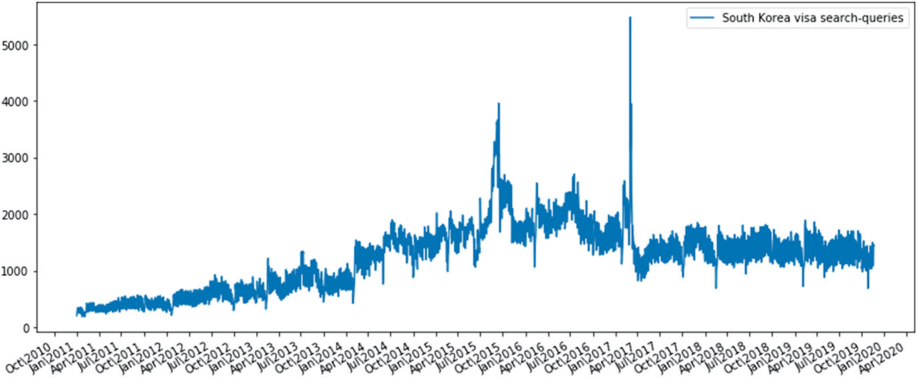
\includegraphics[width=0.8\textwidth]{gfx/m1l1_nowcast_korea_visa_searches.jpg}
    \caption{Baidu: Truy vấn tìm kiếm "Visa Hàn Quốc"}
    \label{fig:nowcast_korea_visa_searches}
\end{figure}

Cuối cùng, bằng cách tổng hợp các xu hướng truy vấn tìm kiếm của những từ khóa đã được xác định đó, Chỉ số Du lịch Trung Quốc tại Hàn Quốc của chúng tôi theo dõi theo thời gian thực sự phát triển của số liệu chính thức về lượng du khách Trung Quốc đến Hàn Quốc. Chúng tôi tính toán sự thay đổi so với cùng kỳ năm trước của chỉ số này và xác nhận nó bằng cách sử dụng các con số chính thức của khách du lịch Trung Quốc tại Hàn Quốc (xem Hình 4).

\begin{figure}[htbp]
    \centering
    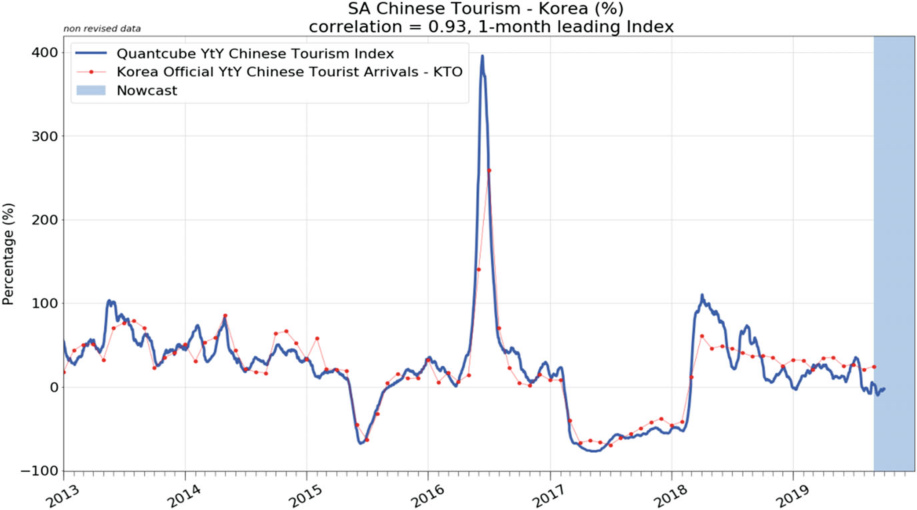
\includegraphics[width=0.8\textwidth]{gfx/m1l1_nowcast_chinese_tourism_korea.jpg}
    \caption{Chỉ số du lịch Trung Quốc tại Hàn Quốc ngắn hạn (so với cùng kỳ năm trước tính bằng \%)}
    \label{fig:nowcast_chinese_tourism_korea}
\end{figure}

Từ Hình 4, chúng ta quan sát thấy rằng Chỉ số Du lịch Trung Quốc QuantCube theo dõi chính xác lượng du khách Trung Quốc đến Hàn Quốc. Ví dụ, chỉ số này đã nắm bắt được sự sụt giảm đầu tiên vào tháng 6 năm 2015 do đợt bùng phát MERS. Hơn nữa, vào năm 2017, sau thông báo về việc lắp đặt Hệ thống phòng thủ khu vực tầm cao giai đoạn cuối (THAAD) hùng mạnh vào cuối năm 2016, chính phủ Trung Quốc đã cấm các nhóm du lịch đến Hàn Quốc như một sự trả đũa kinh tế. Trong toàn bộ năm 2017, Hàn Quốc có 4,2 triệu du khách Trung Quốc – giảm 48,3\% so với năm trước. Sự sụt giảm của khách du lịch Trung Quốc dẫn đến việc lượng khách du lịch nhập cảnh giảm 36\%. Do đó, chỉ báo Du lịch Trung Quốc thời gian thực này cũng rất hữu ích để ước tính trong thời gian thực xu hướng của ngành Du lịch Hàn Quốc. Nó theo dõi lượng du khách Trung Quốc đến với mức tương quan lên đến 95\%.

Cuối cùng, chúng tôi đã phát triển các chỉ số tương tự để theo dõi theo thời gian thực lượng du khách Trung Quốc đến 15 quốc gia được ghé thăm nhiều nhất (Mỹ, Châu Âu, v.v.); chúng tôi nhận được mối tương quan trung bình là 80\% cho các quốc gia được ghé thăm nhiều nhất. Bằng cách tổng hợp các chỉ số đó, chúng tôi có thể xây dựng một chỉ số để theo dõi lượng du khách Trung Quốc trên toàn thế giới, cung cấp một biến đại diện (proxy) tuyệt vời cho chi tiêu của các hộ gia đình Trung Quốc trong lĩnh vực cụ thể này.

\subsubsection{Một Biến đại diện Thời gian thực cho Mức độ Hoạt động}

QuantCube Technology đã phát triển một phương pháp luận dựa trên việc phân tích các hình ảnh vệ tinh Sentinel-2 để phát hiện các cơ sở hạ tầng mới (thương mại, hậu cần, công nghiệp hoặc khu dân cư) và đo lường sự tiến hóa về hình dạng và kích thước của các khu vực đô thị. Tuy nhiên, mức độ hoạt động hoặc mức độ khai thác của các khu vực này khó có thể được xác định bằng cách kiểm tra tòa nhà mà có thể được suy luận từ sự hiện diện của các phương tiện từ các đường phố và bãi đậu xe gần đó. Với mục đích này, QuantCube Technology hợp tác với IRISA đã phát triển một mô hình học sâu (deep learning) để đếm xe cộ từ các hình ảnh vệ tinh lấy từ cảm biến Pleiades ở độ phân giải không gian 50 cm. Trên thực tế, chúng tôi chọn vệ tinh tùy thuộc vào độ phân giải pixel cần thiết cho mỗi ứng dụng.

\paragraph{Hình ảnh Vệ tinh}
Hình ảnh vệ tinh ngày càng trở nên dễ tiếp cận hơn trong những năm gần đây. Đặc biệt, một số vệ tinh công cộng cung cấp khả năng truy cập dễ dàng và miễn phí vào kho lưu trữ hình ảnh của họ, với độ phân giải không gian đủ cao cho nhiều ứng dụng liên quan đến đặc tính đất đai. Ví dụ, dòng vệ tinh Sentinel-2 của Cơ quan Vũ trụ Châu Âu (ESA), được phóng vào ngày 23 tháng 6 năm 2015, cung cấp các hình ảnh đa phổ độ phân giải 10 mét bao phủ toàn thế giới. Chúng tôi phân tích những hình ảnh này để phát hiện cơ sở hạ tầng. Để phát hiện và đếm ô tô, chúng tôi sử dụng hình ảnh VHR (độ phân giải rất cao - very high resolution) có độ phân giải cao hơn thu được từ vệ tinh Pleiades (PHR-1A và PHR-1B), do Cơ quan Vũ trụ Pháp (CNES), Phân phối Airbus DS phóng. Những hình ảnh này là các sản phẩm được làm sắc nét toàn sắc (pan-sharpened) thu được bằng cách kết hợp dữ liệu toàn sắc (panchromatic) 50 cm (70 cm ở thiên để, được lấy mẫu lại ở mức 50 cm) và hình ảnh đa phổ 2 m (RGB khả kiến (đỏ, lục, lam) và các dải hồng ngoại). Chúng bao phủ một khu vực lớn gồm các môi trường không đồng nhất bao gồm nông thôn, rừng, khu dân cư, cũng như các khu công nghiệp, nơi sự xuất hiện của các phương tiện bị ảnh hưởng bởi hiệu ứng đổ bóng và che khuất. Một mặt, một trong những ưu điểm của các ứng dụng dựa trên hình ảnh vệ tinh là khả năng mở rộng thế giới tự nhiên (natural world scalability) của chúng. Và mặt khác, sự tiến hóa và cải tiến của các thuật toán trí tuệ nhân tạo cho phép chúng ta xử lý một lượng lớn thông tin có trong hình ảnh vệ tinh một cách dễ dàng, mang lại một giải pháp chuẩn hóa và tự động hoạt động trên dữ liệu thời gian thực.

\paragraph{Tiền xử lý và Lập mô hình}
Việc phát hiện phương tiện từ hình ảnh vệ tinh là một trường hợp đặc biệt của phát hiện đối tượng vì các đối tượng có tính đồng nhất và rất nhỏ (khoảng 5 đến 8 pixel/phương tiện trong hình ảnh Pleiades) và không xếp chồng lên nhau. Để giải quyết nhiệm vụ này, chúng tôi sử dụng một mô hình có tên là Tiramisu 100 lớp (xem [40]). Đây là một mô hình khá tiết kiệm vì nó chỉ có 9 triệu tham số, so với khoảng 130 triệu của mạng học sâu sơ khai được gọi là VGG19. Mục tiêu của mô hình là khai thác việc tái sử dụng tính năng bằng cách mở rộng kiến trúc DenseNet trong khi tránh sự bùng nổ tính năng (feature explosion). Để huấn luyện mô hình học sâu của chúng tôi, chúng tôi đã tạo một tập dữ liệu huấn luyện bằng cách sử dụng công cụ gán nhãn tương tác cho phép gán nhãn 60\% số lượng phương tiện chỉ bằng một cú nhấp chuột sử dụng các phương pháp flood-fill được điều chỉnh cho ứng dụng này. Tập dữ liệu được tạo chứa 87.000 phương tiện được chú thích từ các môi trường khác nhau tùy thuộc vào mức độ đô thị hóa. Từ việc phân đoạn, ước tính về số lượng phương tiện được tính toán dựa trên kích thước và hình dạng của các dự đoán.

\paragraph{Chỉ số Mức độ Hoạt động QuantCube}
Cuối cùng, mô hình thực hiện một dự đoán thỏa mãn đối với ứng dụng phát hiện và đếm phương tiện vì độ chính xác (precision) đạt hơn 85\% trên tập xác thực (validation set) gồm 2673 phương tiện thuộc các khu đô thị và công nghiệp. Thuật toán hiện tại có khả năng xử lý các môi trường đô thị khác nhau. Như có thể thấy trong Hình 5, hiển thị toàn cảnh khu vực Orly gần Paris, bao gồm dự đoán về việc phát hiện và đếm xe ô tô bằng màu vàng, mã có khả năng đếm chính xác số lượng phương tiện ở một số khu vực được xác định. Ví dụ trong Hình 5 cho thấy số lượng phương tiện cho mỗi hộp giới hạn (bounding box) được xác định tương ứng với bãi đậu xe của các địa điểm khách sạn, thương mại hoặc hậu cần (logistics). Bắt đầu từ thông tin dựa trên vệ tinh này, chúng tôi có thể tính toán một chỉ số để phát hiện và đếm số lượng phương tiện ở các địa điểm được xác định và để theo dõi mức độ hoạt động hoặc mức độ khai thác của chúng bằng cách xem xét sự phát triển của chỉ số tương quan với các chỉ số bán hàng. Sử dụng hình ảnh vệ tinh, nó cho phép tạo ra một phương pháp luận và các thước đo chuẩn hóa về mức độ hoạt động cho phép các tổ chức tài chính và các nhóm công ty dự đoán các xu hướng đầu tư mới trước khi công bố các con số kinh tế chính thức.

\begin{figure}[htbp]
    \centering
    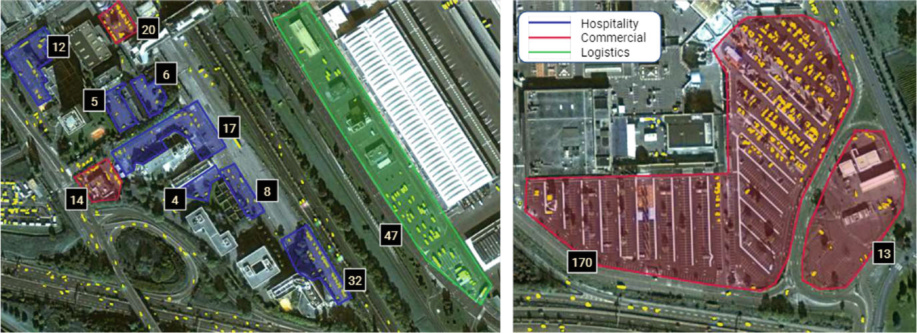
\includegraphics[width=0.8\textwidth]{gfx/m1l1_nowcast_satellite_parking.jpg}
    \caption{Số lượng xe theo từng khu vực ở Orly}
    \label{fig:nowcast_satellite_parking}
\end{figure}

